\documentclass[12pt]{article}
\usepackage[margin=1in]{geometry} 
\usepackage{amsmath,amsthm,amssymb}
\usepackage{xcolor}
\usepackage{listings}
\usepackage{cases}
\usepackage{graphicx}
\usepackage[hidelinks]{hyperref}
\lstset{basicstyle=\ttfamily,
  showstringspaces=false,
  commentstyle=\color{red},
  keywordstyle=\color{blue}
}
\DeclareMathOperator{\B}{\mathbf{B}}
\DeclareMathOperator{\C}{\mathbf{C}}
\DeclareMathOperator{\A}{\mathbf{A}}
\DeclareMathOperator{\T}{\mathbf{T}}
\DeclareMathOperator{\D}{\Delta}
\DeclareMathOperator{\al}{\mathbf{\alpha}}
\DeclareMathOperator{\Th}{\mathbf{\theta}}
\graphicspath{{./figs/}}
 
\title{Project \#2}
\author{Shao Hua, Huang\\
ICN5534 - Robotics}

\begin{document}
\maketitle
\section{Language and Platform Description}
\begin{enumerate}
  \item
  I use C\texttt{++} and Python3 to write my program.\\
  If possible, please use linux machine to run my code.
  \begin{enumerate}
    \item C\texttt{++}11 feature is required.
    \item Eigen: C\texttt{++} template library for linear algebra
    \item python packages: numpy and matplotlib
  \end{enumerate}
  \item Intall Dependencies\\
  Eigen3: \lstinline{sudo apt install libeigen3-dev}\\
  numpy and matplotlib: \lstinline{pip3 install numpy matplotlib}
  \item Run
  \begin{lstlisting}[language=bash]
python3 project2.py
  \end{lstlisting}
\end{enumerate}
\section{Program Architecture}
\begin{enumerate}
  \item project1.hpp and project1.cc: codes from project1
    \begin{itemize}
      \item IsValidRange: check if the angle is not NaN and is in valid range
      \item MakeVector6: make a 6 x 1 vector in Eigen
      \item MakeA: given $(d_n, a_n, \al_n, \Th_n)$, make matrix $\A_n$
      \item DoTask1: given $(n, o, a, p)$, compute joint variables
      \item DoTask2: given joint variables, compute $(n, o, a, p)$ and $(x, y, z, \phi, \Th, \phi)$
      \item PrintAnswer: print task1 answer for command line interface
    \end{itemize}
  \item project2.py
    \begin{itemize}
      \item path\_planning: path planning algorithm from textbook
      \item plot\_param: plot position/angle, velocity, accerlation parameters
      \item plot\_3dpath: plot final 3d path
    \end{itemize}
\end{enumerate}
\section{Equations Derivation}
\begin{numcases}{}
  a_4t_{acc}^4 + a_3t_{acc}^3 + a_2t_{acc}^2 + a_1t_{acc} + a_0 = \B + \D \C \frac{t_{acc}}{\T}\label{eq1}\\
  a_4t_{acc}^4 - a_3t_{acc}^3 + a_2t_{acc}^2 - a_1t_{acc} + a_0 = \B + \D \B\label{eq2}\\
  4a_4t_{acc}^3 + 3a_3t_{acc}^2 + 2a_2t_{acc} + a_1 = \frac{\D\C}{\T}\label{eq3}\\
  -4a_4t_{acc}^3 + 3a_3t_{acc}^2 - 2a_2t_{acc} + a_1 = -\frac{\D\B}{t_{acc}}\label{eq4}\\
  12a_4t_{acc}^2 + 3a_3t_{acc} + 2a_2 = 0\label{eq5}\\
  12a_4t_{acc}^2 - 3a_3t_{acc} + 2a_2 = 0\label{eq6}
\end{numcases}
\begin{align}
\text{from } \eqref{eq5} \text{ and } \eqref{eq6} & \Rightarrow a_3 = 0\\
\eqref{eq1} - \eqref{eq2} & \Rightarrow a_1 = \frac{1}{2t_{acc}}(\D\C\frac{t_{acc}}{\T}-\D\B) = \frac{1}{2t_{acc}}(\D\C\frac{t_{acc}}{\T}+\D\B)-\frac{1}{t_{acc}}\D\B\\
\eqref{eq3} * 3 & \Rightarrow 12a_4t_{acc}^2 + 6a_2 = \frac{3}{2t_{acc}^2}(\D\C\frac{t_{acc}}{\T}+\D\B)\label{eq7}\\
\eqref{eq7} - \eqref{eq5} & \Rightarrow a_2 = \frac{3}{8t_{acc}^2}(\D\C\frac{t_{acc}}{\T}+\D\B)\label{eq8}\\
\text{sub } \eqref{eq8} \text{ to } \eqref{eq5} & \Rightarrow a_4 = -\frac{1}{16t_{acc}^4}(\D\C\frac{t_{acc}}{\T}+\D\B)\\
\text{sub to } \eqref{eq1} & \Rightarrow a_0 = \frac{3}{16}(\D\C\frac{t_{acc}}{\T}+\D\B) + \B
\end{align}
Let $$h = \frac{t + t_{acc}}{2t_{acc}}$$
Then,
\begin{align*}
q(t) & = (\D\C\frac{t_{acc}}{\T}+\D\B)(-\frac{t^4}{16t_{acc}^4}+\frac{3t^2}{8t_{acc}^2}+\frac{t}{2t_{acc}}+\frac{3}{16})+\B-\frac{t}{t_{acc}}\D\B\\
     & = (\D\C\frac{t_{acc}}{\T}+\D\B)(2-h)h^3 + \B + (1-2h)\D\B\\
\dot{q}(t) & = (\D\C\frac{t_{acc}}{\T}+\D\B)(-\frac{t^3}{4t_{acc}^4}+\frac{3t}{4t_{acc}^2}+\frac{1}{2t_{acc}})-\frac{1}{t_{acc}}\D\B\\
           & = \left[(\D\C\frac{t_{acc}}{\T}+\D\B)(3-2h)h^2-\D\B\right]\frac{1}{t_{acc}}\\
\ddot{q}(t) & = (\D\C\frac{t_{acc}}{\T}+\D\B)(-\frac{3t^2}{4t_{acc}^4}+\frac{3}{4t_{acc}^2})\\
            & = (\D\C\frac{t_{acc}}{\T}+\D\B)(1-h)\frac{3h}{t_{acc}^2}
\end{align*}
\section{Result}
\subsection{Joint Motion}
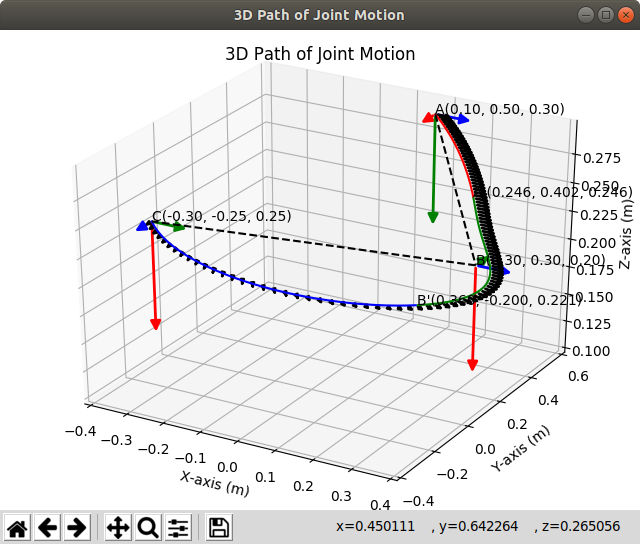
\includegraphics[scale=0.5]{joint_path}\\
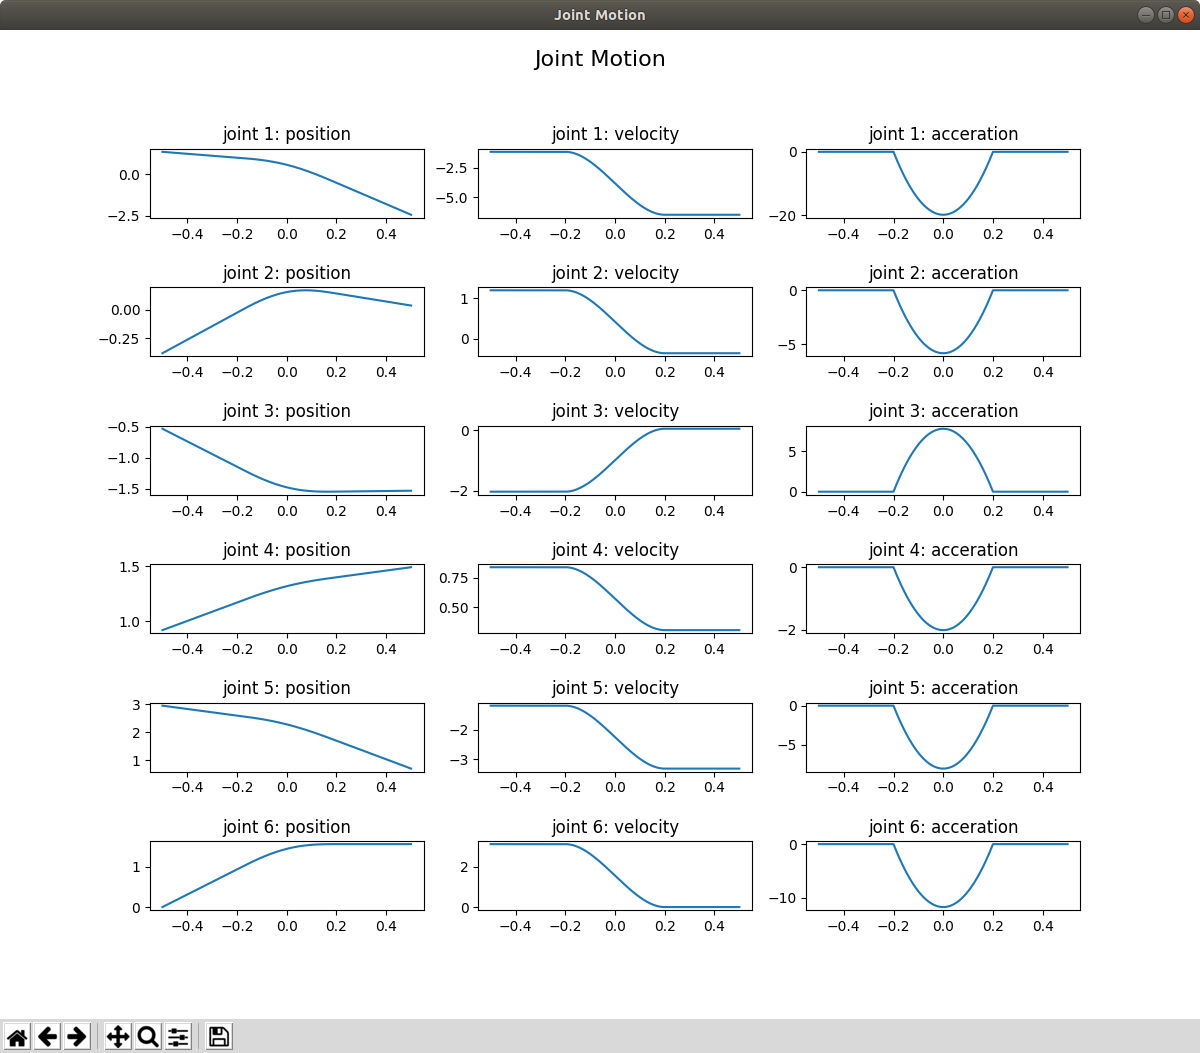
\includegraphics[scale=0.3]{joint_param}
\subsection{Cartesian Motion}
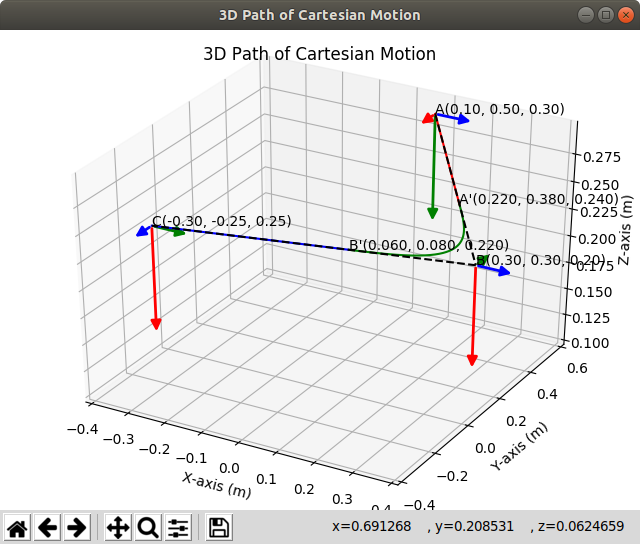
\includegraphics[scale=0.5]{cartesian_path}\\
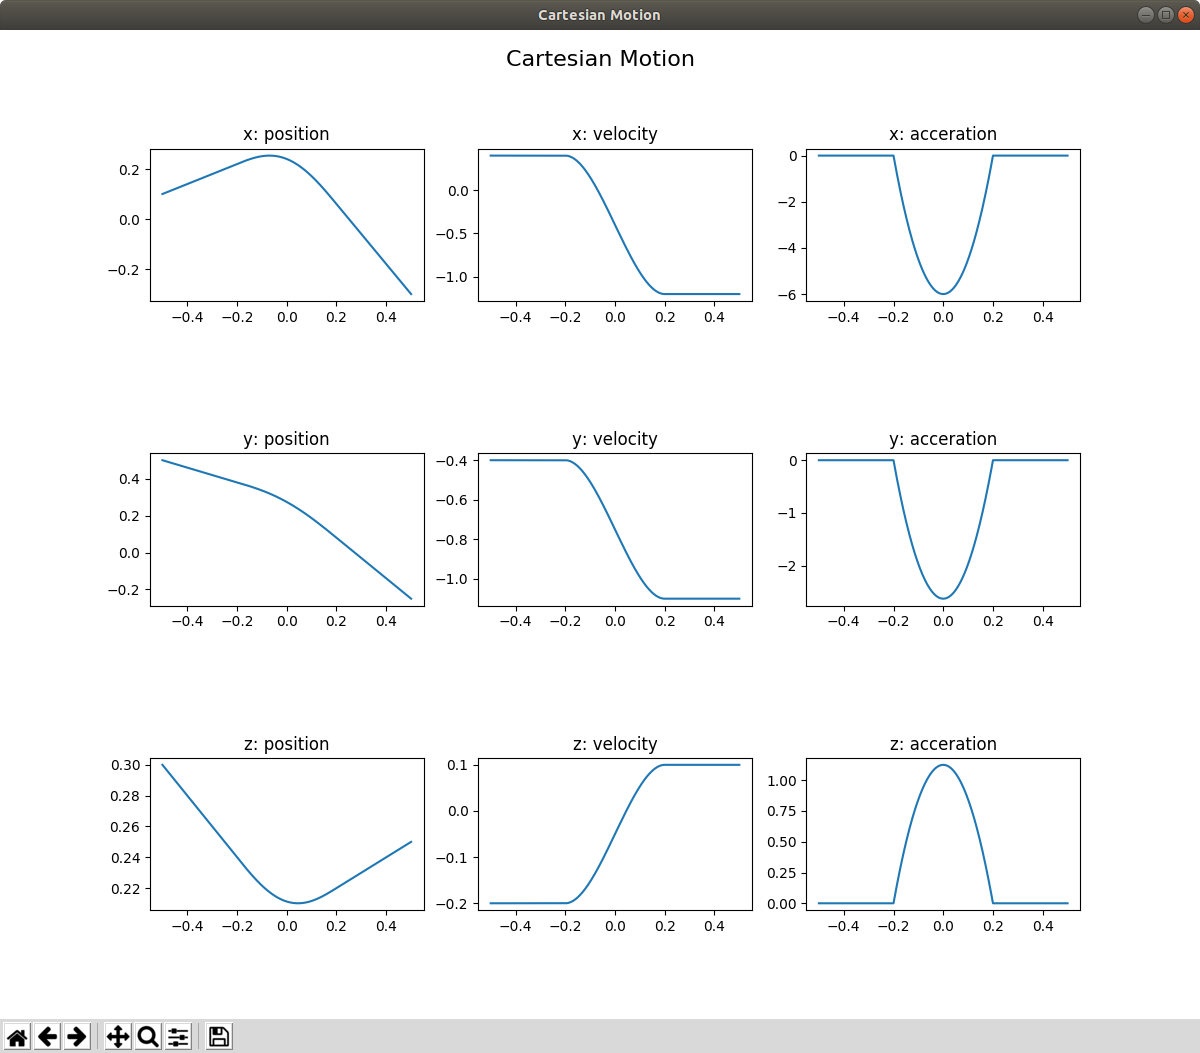
\includegraphics[scale=0.3]{cartesian_param}
\section{Difference Between Joint and Cartesian Motion}
\subsection{Joint Motion}
\begin{enumerate}
  \item Pros
  \begin{itemize}
    \item Efficient in computation
    \item No singularity problem
    \item No configuration problem
    \item Minimum time planning
  \end{itemize}
  \item Cons: The corresponding Cartesian locations may be complicated.
\end{enumerate}
\subsection{Cartesian Motion}
\begin{enumerate}
  \item Pros
  \begin{itemize}
    \item Motion between path segments and points is well defined.
    \item Different constraints, such as smoothness and shortest path, etc., can be imposed upon.
  \end{itemize}
  \item Cons
  \begin{itemize}
    \item Computational load is high.
    \item The motion breaks down when singularity occurs.
  \end{itemize}
\end{enumerate}
\end{document}
